

\subsection{Komplexe Zahlen}

\begin{examplecode}{Komplexe Zahlen in Python}
\begin{lstlisting}[language=Python, style=basesmol]
def complex_operations(z1, z2):
    """Grundlegende Operationen mit komplexen Zahlen."""
    # Basisfunktionen
    def to_polar(z):
        r = (z.real**2 + z.imag**2)**0.5
        phi = math.atan2(z.imag, z.real)
        return r, phi
    
    def from_polar(r, phi):
        return r * (math.cos(phi) + 1j*math.sin(phi))
    
    try:
        # Addition und Subtraktion
        z_add = z1 + z2
        z_sub = z1 - z2
        
        # Multiplikation und Division
        z_mul = z1 * z2
        z_div = z1 / z2 if z2 != 0 else None
        
        # Polarform
        r1, phi1 = to_polar(z1)
        r2, phi2 = to_polar(z2)
        
        # Exponentialform
        z1_exp = from_polar(r1, phi1)
        z2_exp = from_polar(r2, phi2)
        
        return {
            'addition': z_add,
            'subtraktion': z_sub,
            'multiplikation': z_mul,
            'division': z_div,
            'polar_z1': (r1, phi1),
            'polar_z2': (r2, phi2)
        }
        
    except Exception as e:
        print(f"Fehler bei Berechnung: {e}")
        return None

# Beispiel
z1 = 3 - 11j
z2 = 2 + 5j
results = complex_operations(z1, z2)
\end{lstlisting}
\end{examplecode}

\columnbreak

\section{Komplexe Zahlen}

\begin{lemma}{Fundamentalsatz der Algebra}\\
Eine algebraische Gleichung n-ten Grades mit komplexen Koeffizienten:
$$a_nz^n + a_{n-1}z^{n-1} + \cdots + a_1z + a_0 = 0$$
besitzt in $\mathbb{C}$ genau n Lösungen (mit Vielfachheiten gezählt).
\end{lemma}

\begin{concept}{Komplexe Zahlen}\\
Die Menge der komplexen Zahlen $\mathbb{C}$ erweitert die reellen Zahlen $\mathbb{R}$ durch Einführung der imaginären Einheit $i$ mit der Eigenschaft:
$$i^2 = -1$$

Eine komplexe Zahl $z$ ist ein geordnetes Paar $(x,y)$ mit $x,y \in \mathbb{R}$:
$$z = x + iy$$

Die Menge aller komplexen Zahlen ist definiert als:
$$\mathbb{C} = \{z \mid z = x + iy \text{ mit } x,y \in \mathbb{R}\}$$
\end{concept}

\begin{definition}{Bestandteile komplexer Zahlen}\\
\begin{minipage}[t]{0.6\textwidth}
    \vspace{-7mm}
    \textbf{Realteil:} $\operatorname{Re}(z) = x$\\
    \textbf{Imaginärteil:} $\operatorname{Im}(z) = y$\\
    \textbf{Betrag:} $|z| = \sqrt{x^2 + y^2} = \sqrt{z \cdot z^*}$\\
    \textbf{Konjugation:} $\overline{z} = x - iy$
\end{minipage}
\begin{minipage}{0.35\textwidth}
    \vspace{-3mm}
    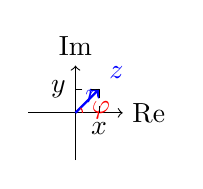
\begin{tikzpicture}[scale=0.3]
        % Coordinate axes
        \draw[->] (-2,0) -- (2,0) node[right] {Re};
        \draw[->] (0,-2) -- (0,2) node[above] {Im};
        
        % Example point and vector
        \draw[thick,blue,->] (0,0) -- (1,1) node[above right] {$z$};
        
        % Angle and labels
        \draw[red] (0.3,0) arc (0:45:0.3) node[midway,right] {$\varphi$};
        
        % Components
        \draw[dashed] (1,1) -- (1,0) node[below] {$x$};
        \draw[dashed] (1,1) -- (0,1) node[left] {$y$};
        
        % Radius
        \node[blue] at (0.7,0.7) {$r$};
    \end{tikzpicture}
\end{minipage}
\end{definition}

\begin{theorem}{Rechenoperationen mit komplexen Zahlen}\\
Für $z_1 = x_1 + iy_1$ und $z_2 = x_2 + iy_2$ gilt:
\vspace{1mm}\\
\begin{minipage}[t]{0.45\textwidth}
    \textbf{Addition:}\\
    $z_1 + z_2 = (x_1 + x_2) + i(y_1 + y_2)$
\end{minipage}
\hspace{3mm}
\begin{minipage}[t]{0.45\textwidth}
    \textbf{Subtraktion:}\\
    $z_1 - z_2 = (x_1 - x_2) + i(y_1 - y_2)$
\end{minipage}

\vspace{2mm}
\textbf{Multiplikation:}
\begin{align*}
    z_1 \cdot z_2 &= (x_1x_2 - y_1y_2) + i(x_1y_2 + x_2y_1)\\
    &= r_1r_2e^{i(\varphi_1 + \varphi_2)} \text{ (in Exponentialform)}
\end{align*}

\textbf{Division:}
\begin{align*}
    \frac{z_1}{z_2} &= \frac{z_1 \cdot z_2^*}{z_2 \cdot z_2^*} = \frac{(x_1x_2 + y_1y_2) + i(y_1x_2 - x_1y_2)}{x_2^2 + y_2^2}\\
    &= \frac{r_1}{r_2}e^{i(\varphi_1 - \varphi_2)} \text{ (in Exponentialform)}
\end{align*}
\end{theorem}

\begin{theorem}{Potenzen und Wurzeln}\\
Für eine komplexe Zahl in Exponentialform $z = re^{i\varphi}$ gilt:
\begin{itemize}
    \item n-te Potenz: $z^n = r^ne^{in\varphi} = r^n(\cos(n\varphi) + i\sin(n\varphi))$
    \item n-te Wurzel: $z_k = \sqrt[n]{r}e^{i\frac{\varphi + 2\pi k}{n}}$, $k = 0,1,\ldots,n-1$
\end{itemize}
\end{theorem}

\begin{concept}{Darstellungsformen}
\begin{itemize}
    \item Normalform: $z = x + iy$
    \item Trigonometrische Form: $z = r(\cos\varphi + i\sin\varphi)$
    \item Exponentialform: $z = re^{i\varphi}$
\end{itemize}
$x = r\cos\varphi, \quad y = r\sin\varphi, \quad r = \sqrt{x^2 + y^2}\\
    \varphi = \arcsin\left(\frac{y}{r}\right) = \arccos\left(\frac{x}{r}\right)\\
    e^{i\varphi} = \cos\varphi + i\sin\varphi \text{ (Euler-Formel)}$

\end{concept}

\begin{KR}{Umrechnung zwischen Darstellungsformen komplexer Zahlen}
\paragraph{Von Normalform in trigonometrische Form/Exponentialform}
\begin{enumerate}
   \item Berechne Betrag $r = \sqrt{x^2 + y^2}$
   \item Berechne Winkel mit einer der Formeln: 
   \begin{itemize}
       \item $\varphi = \arctan(\frac{y}{x})$ falls $x > 0$
       \item $\varphi = \arctan(\frac{y}{x}) + \pi$ falls $x < 0$
       \item $\varphi = \frac{\pi}{2}$ falls $x = 0, y > 0$
       \item $\varphi = -\frac{\pi}{2}$ falls $x = 0, y < 0$
       \item $\varphi$ unbestimmt falls $x = y = 0$
   \end{itemize}
   \item Trigonometrische Form: $z = r(\cos\varphi + i\sin\varphi)$
   \item Exponentialform: $z = re^{i\varphi}$
\end{enumerate}

\paragraph{Von trigonometrischer Form in Normalform}
\begin{enumerate}
   \item Realteil: $x = r\cos\varphi$
   \item Imaginärteil: $y = r\sin\varphi$
   \item Normalform: $z = x + iy$
\end{enumerate}

\paragraph{Von Exponentialform in Normalform/trigonometrische Form}
\begin{enumerate}
   \item Trigonometrische Form durch Euler-Formel:\\
   $re^{i\varphi} = r(\cos\varphi + i\sin\varphi)$
   \item Dann wie oben in Normalform umrechnen
\end{enumerate}

\paragraph{Wichtige Hinweise:}
\begin{itemize}
   \item Achten Sie auf das korrekte Quadranten beim Winkel
   \item Winkelfunktionen im Bogenmaß verwenden
   \item Bei Umrechnung in Normalform Euler-Formel nutzen
   \item Vorzeichen bei Exponentialform beachten
\end{itemize}
\end{KR}


\begin{example2}{Darstellungsformen}
Gegeben: $z = 3 - 11i$ in Normalform
$$r = \sqrt{3^2 + 11^2} = \sqrt{130}, \quad \varphi = \arcsin(\frac{11}{\sqrt{130}}) = 1.3 \text{rad} = 74.74^{\circ}$$
\textbf{Trigonometrische Form:} $z = \sqrt{130}(\cos(1.3) + i\sin(1.3))$
\vspace{2mm}\\
\textbf{Exponentialform:} $z = \sqrt{130}e^{i\cdot 1.3}$
\end{example2}


\section{Eigenwerte und Eigenvektoren}

\begin{definition}{Eigenwerte und Eigenvektoren}\\
Für eine Matrix $A \in \mathbb{R}^{n\times n}$ heißt $\lambda \in \mathbb{C}$ Eigenwert von $A$, wenn es einen Vektor $x \in \mathbb{C}^n \backslash \{0\}$ gibt mit:
\vspace{-2mm}\\
$$Ax = \lambda x$$
Der Vektor $x$ heißt dann Eigenvektor zum Eigenwert $\lambda$.
\end{definition}

\begin{concept}{Bestimmung von Eigenwerten}\\
Ein Skalar $\lambda$ ist genau dann Eigenwert von $A$, wenn gilt:
\vspace{-2mm}\\
$$\det(A - \lambda I_n) = 0$$
Diese Gleichung heißt charakteristische Gleichung. Das zugehörige Polynom
\vspace{-2mm}
$$p(\lambda) = \det(A - \lambda I_n)$$
ist das charakteristische Polynom von $A$.
\end{concept}

\begin{theorem}{Eigenschaften von Eigenwerten}
Für eine Matrix $A \in \mathbb{R}^{n\times n}$ gilt:
\begin{itemize}
    \item $\det(A) = \prod_{i=1}^n \lambda_i$ (Produkt der Eigenwerte)
    \item $\operatorname{tr}(A) = \sum_{i=1}^n \lambda_i$ (Summe der Eigenwerte)
    \item Bei Dreiecksmatrix sind die Diagonalelemente die Eigenwerte
    \item Ist $\lambda$ Eigenwert von $A$, so ist $\frac{1}{\lambda}$ Eigenwert von $A^{-1}$
\end{itemize}
\end{theorem}

\begin{concept}{Vielfachheiten}
Für einen Eigenwert $\lambda$ unterscheidet man:
\begin{itemize}
    \item Algebraische Vielfachheit: \\Vielfachheit als Nullstelle des charakteristischen Polynoms
    \item Geometrische Vielfachheit: \\Dimension des Eigenraums $= n - \operatorname{rg}(A-\lambda I_n)$
\end{itemize}
Die geometrische Vielfachheit ist stets kleiner oder gleich der algebraischen Vielfachheit.
\end{concept}

\begin{KR}{Bestimmung von Eigenwerten und Eigenvektoren}
\begin{enumerate}
    \item Charakteristisches Polynom aufstellen: 
    \begin{itemize}
        \item Matrix $(A-\lambda I_n)$ bilden
        \item Determinante berechnen: $p(\lambda) = \det(A-\lambda I_n)$
    \end{itemize}
    \item Eigenwerte bestimmen:
    \begin{itemize}
        \item $p(\lambda) = 0$ lösen
        \item Bei Dreiecksmatrix: Diagonalelemente sind Eigenwerte
    \end{itemize}
    \item Für jeden Eigenwert $\lambda_i$:
    \begin{itemize}
        \item System $(A-\lambda_i I_n)x = 0$ aufstellen
        \item Gaussverfahren anwenden 
        \item Lösungsraum = Eigenraum bestimmen
        \item Basis des Eigenraums = linear unabhängige Eigenvektoren
        \item Lösung parametrisieren
        \item Parameter != 0 waehlen für Eigenvektor
    \end{itemize}
    \item Überprüfung:
    \begin{itemize}
        \item $Ax = \lambda x$ für jeden Eigenvektor
        \item Anzahl linear unabhaengiger Eigenvektoren kleiner als algebraische Vielfachheit
    \end{itemize}
\end{enumerate}
\end{KR}



\begin{example2}{Eigenwertberechnung}
Gegeben ist die Matrix
$A = \begin{psmallmatrix} 
2 & 1 & 0 \\
1 & 2 & 1 \\
0 & 1 & 2
\end{psmallmatrix}$

1. Charakteristisches Polynom aufstellen:\\
   $\det(A - \lambda I) = \begin{vsmallmatrix} 
   2-\lambda & 1 & 0 \\
   1 & 2-\lambda & 1 \\
   0 & 1 & 2-\lambda
   \end{vsmallmatrix}$
   \vspace{1mm}\\
2. Entwicklung nach 1. Zeile:
   $p(\lambda) = (2-\lambda)\begin{vsmallmatrix}
   2-\lambda & 1 \\
   1 & 2-\lambda
   \end{vsmallmatrix} - 1\begin{vsmallmatrix}
   1 & 1 \\
   1 & 2-\lambda
   \end{vsmallmatrix}$
   \vspace{1mm}\\
3. Ausrechnen:\\
   $p(\lambda) = (2-\lambda)((2-\lambda)^2 - 1) - ((2-\lambda) - 1)$
   $= -\lambda^3 + 6\lambda^2 - 11\lambda + 6$
   \vspace{1mm}\\
4. Nullstellen bestimmen:
   $\lambda_1 = 1, \lambda_2 = 2, \lambda_3 = 3$
\vspace{1mm}\\
5. Eigenvektoren bestimmen für $\lambda_1 = 1$:\\
   $(A - I)x = 0$ führt zu $x_1 = \begin{psmallmatrix} 1 \\ -2 \\ 1 \end{psmallmatrix}$
\end{example2}

\begin{examplecode}{Charakteristisches Polynom und Eigenwerte}
\begin{lstlisting}[language=Python, style=basesmol]
def det_2x2(matrix):
    return matrix[0][0]*matrix[1][1] - matrix[0][1]*matrix[1][0]

def det_3x3(matrix):
    det = 0
    # Entwicklung nach erster Zeile
    for i in range(3):
        minor = []
        for j in range(1,3):
            row = []
            for k in range(3):
                if k != i:
                    row.append(matrix[j][k])
            minor.append(row)
        det += ((-1)**i) * matrix[0][i] * det_2x2(minor)
    return det

def char_poly_coeff(matrix):
    """Berechnet Koeffizienten des charakteristischen Polynoms"""
    n = len(matrix)
    coeffs = [0] * (n+1)
    
    # Lambda^n Koeffizient
    coeffs[n] = (-1)**n
    
    # Spur (Lambda^(n-1) Koeffizient)
    trace = sum(matrix[i][i] for i in range(n))
    coeffs[n-1] = (-1)**(n-1) * trace
    
    # Determinante (konstanter Term)
    coeffs[0] = det_3x3(matrix)
    
    return coeffs

# Beispielmatrix
A = [[2, 1, 0],
     [1, 2, 1],
     [0, 1, 2]]

# Charakteristisches Polynom berechnen
poly = char_poly_coeff(A)
print("Charakteristisches Polynom:")
print(f"p(lambda) = lambda^3 {poly[2]:+}lambda^2 {poly[1]:+}lambda {poly[0]:+}")
\end{lstlisting}
\end{examplecode}

\begin{examplecode}{Eigenvektoren berechnen}
\begin{lstlisting}[language=Python, style=basesmol]
def gauss_elimination(A, b):
    """Loest Ax=b mit Gauss-Elimination"""
    n = len(A)
    # Erweiterte Matrix erstellen
    M = [[A[i][j] for j in range(n)] + [b[i]] for i in range(n)]
    
    # Vorwaertselimination
    for i in range(n):
        pivot = M[i][i]
        if abs(pivot) < 1e-10:
            continue
        for j in range(i+1, n):
            factor = M[j][i] / pivot
            for k in range(i, n+1):
                M[j][k] -= factor * M[i][k]
    
    # Rueckwaertssubstitution
    x = [0] * n
    for i in range(n-1, -1, -1):
        if abs(M[i][i]) < 1e-10:
            x[i] = 1  # Freie Variable
            continue
        sum_val = sum(M[i][j] * x[j] for j in range(i+1, n))
        x[i] = (M[i][n] - sum_val) / M[i][i]
    
    return x

def find_eigenvector(A, eigenvalue):
    """Findet Eigenvektor zum Eigenwert"""
    n = len(A)
    # A - lambda*I
    A_lambda = [[A[i][j] - (eigenvalue if i==j else 0) 
                for j in range(n)] for i in range(n)]
    
    # Loese (A - lambda*I)x = 0
    b = [0] * n
    return gauss_elimination(A_lambda, b)

# Eigenvektoren fuer lambda = 1,2,3 berechnen
eigenvalues = [1, 2, 3]
for ev in eigenvalues:
    vec = find_eigenvector(A, ev)
    print(f"Eigenvektor fuer lambda={ev}:", vec)
\end{lstlisting}
\end{examplecode}



\subsubsection{Numerische Berechnung von Eigenwerten}

\begin{concept}{Ähnliche Matrizen}\\
Zwei Matrizen $A,B \in \mathbb{R}^{n\times n}$ heißen ähnlich, wenn es eine reguläre Matrix $T$ gibt mit:
$$B = T^{-1}AT$$

Eine Matrix $A$ heißt diagonalisierbar, wenn sie ähnlich zu einer Diagonalmatrix $D$ ist:
$$D = T^{-1}AT$$
\end{concept}

\begin{theorem}{Eigenschaften ähnlicher Matrizen}\\
Für ähnliche Matrizen $A$ und $B = T^{-1}AT$ gilt:
\begin{enumerate}
    \item $A$ und $B$ haben dieselben Eigenwerte mit gleichen algebraischen Vielfachheiten
    \item Ist $x$ Eigenvektor von $B$ zum Eigenwert $\lambda$, so ist $Tx$ Eigenvektor von $A$ zum Eigenwert $\lambda$
    \item Bei Diagonalisierbarkeit:
    \begin{itemize}
        \item Die Diagonalelemente von $D$ sind die Eigenwerte von $A$
        \item Die Spalten von $T$ sind die Eigenvektoren von $A$
    \end{itemize}
\end{enumerate}
\end{theorem}

\begin{definition}{Spektralradius}
Der Spektralradius einer Matrix $A$ ist definiert als:
$$\rho(A) = \max\{|\lambda| \mid \lambda \text{ ist Eigenwert von } A\}$$
Er gibt den Betrag des betragsmäßig größten Eigenwerts an.
\end{definition}

\subsubsection{Von-Mises-Iteration}

\begin{concept}{Von-Mises-Iteration (Vektoriteration)}\\
Für eine diagonalisierbare Matrix $A$ mit Eigenwerten $|\lambda_1| > |\lambda_2| \geq \cdots \geq |\lambda_n|$ konvergiert die Folge:
$$v^{(k+1)} = \frac{Av^{(k)}}{\|Av^{(k)}\|_2}, \quad
\lambda^{(k+1)} = \frac{(v^{(k)})^TAv^{(k)}}{(v^{(k)})^Tv^{(k)}}$$
gegen einen Eigenvektor $v$ zum betragsmäßig größten Eigenwert $\lambda_1$.
\end{concept}

\begin{KR}{Von-Mises-Iteration durchführen}
\begin{enumerate}
    \item Wähle Startvektor $v^{(0)}$ mit $\|v^{(0)}\|_2 = 1$
    \item Für $k = 0,1,2,\ldots$:
    \begin{itemize}
        \item Berechne $w^{(k)} = Av^{(k)}$
        \item Normiere: $v^{(k+1)} = \frac{w^{(k)}}{\|w^{(k)}\|_2}$
        \item Berechne Rayleigh-Quotienten $\lambda^{(k+1)}$
        \item Prüfe Konvergenz
    \end{itemize}
\end{enumerate}
\end{KR}

\begin{example2}{Von-Mises-Iteration}
Berechne größten Eigenwert der Matrix:
$$A = \begin{psmallmatrix}
4 & -1 & 1\\
-1 & 3 & -2\\
1 & -2 & 3
\end{psmallmatrix}$$

Startvektor: $v^{(0)} = \begin{psmallmatrix}1\\ 0\\ 0\end{psmallmatrix}$

\begin{center}
\begin{tabular}{c|c|c}
k & $v^{(k)}$ & $\lambda^{(k)}$ \\\hline
0 & $(1, 0, 0)^T$ & -\\
1 & $(0.970, -0.213, 0.119)^T$ & 4.000\\
2 & $(0.957, -0.239, 0.164)^T$ & 4.827\\
3 & $(0.953, -0.244, 0.178)^T$ & 4.953\\
4 & $(0.952, -0.245, 0.182)^T$ & 4.989
\end{tabular}
\end{center}

Konvergenz gegen $\lambda_1 \approx 5$ mit Eigenvektor $v \approx (0.952, -0.245, 0.182)^T$
\end{example2}

\begin{examplecode}{Von-Mises-Iteration} Berechnung des größten Eigenwerts
    %TODO: check if this is correct
\begin{lstlisting}[language=Python, style=basesmol]
def power_iteration(A, tol=1e-10, max_iter=100):
    n = len(A)
    v = [random.random() for _ in range(n)]
    v = [x / np.linalg.norm(v) for x in v]
    for i in range(max_iter):
        w = [sum(A[i][j] * v[j] for j in range(n)) for i in range(n)]
        v_new = [x / np.linalg.norm(w) for x in w]
        # Rayleigh-Quotient
        lambda_k = sum(v_new[i] * A[i][j] * v_new[j] for i in range(n) for j in range(n))
        if np.linalg.norm([v_new[i] - v[i] for i in range(n)]) < tol:
            return lambda_k, v_new
        v = v_new
    return lambda_k, v_new
\end{lstlisting}
\end{examplecode}

\begin{examplecode}{Von-Mises-Iteration}
\begin{lstlisting}[language=Python, style=basesmol]
def matrix_vector_mult(A, v):
    n = len(v)
    return [sum(A[i][j] * v[j] for j in range(n)) 
            for i in range(n)]

def vector_norm(v):
    return (sum(x*x for x in v)) ** 0.5

def normalize_vector(v):
    norm = vector_norm(v)
    return [x/norm for x in v]

def rayleigh_quotient(A, v):
    numerator = sum(v[i] * sum(A[i][j] * v[j] 
                   for j in range(len(v))) 
                   for i in range(len(v)))
    denominator = sum(x*x for x in v)
    return numerator / denominator

def power_method(A, tol=1e-10, max_iter=100):
    n = len(A)
    # Startvektor [1,0,0,...,0]
    v = [1.0] + [0.0] * (n-1)
    v = normalize_vector(v)
    
    for k in range(max_iter):
        # Matrixmultiplikation
        w = matrix_vector_mult(A, v)
        # Normierung
        v_new = normalize_vector(w)
        # Eigenwertapproximation
        lambda_k = rayleigh_quotient(A, v_new)
        # Konvergenztest
        if vector_norm([v_new[i]-v[i] 
                     for i in range(n)]) < tol:
            return lambda_k, v_new
        v = v_new
    
    return lambda_k, v
\end{lstlisting}
\end{examplecode}

\begin{examplecode}{Von-Mises-Iteration ohne spezielle Bibliotheken}
\begin{lstlisting}[language=Python, style=basesmol]
def matrix_vector_mult(A, v):
    n = len(A)
    result = [0] * n
    for i in range(n):
        for j in range(n):
            result[i] += A[i][j] * v[j]
    return result

def vector_norm(v):
    return sum(x*x for x in v) ** 0.5

def normalize_vector(v):
    norm = vector_norm(v)
    return [x/norm for x in v]

def power_iteration(A, tol=1e-10, max_iter=100):
    n = len(A)
    # Startvektor
    v = normalize_vector([1] + [0]*(n-1))
    
    for _ in range(max_iter):
        # Matrix-Vektor-Multiplikation
        w = matrix_vector_mult(A, v)
        # Normierung
        v_new = normalize_vector(w)
        
        # Rayleigh-Quotient
        lambda_k = sum(v_new[i] * A[i][j] * v_new[j] 
                      for i in range(n) 
                      for j in range(n))
        
        # Konvergenzpruefung
        if vector_norm([v_new[i]-v[i] for i in range(n)]) < tol:
            return lambda_k, v_new
            
        v = v_new
    return lambda_k, v
\end{lstlisting}
\end{examplecode}

\subsubsection{QR-Verfahren}

\begin{concept}{QR-Verfahren}\\
Das QR-Verfahren transformiert die Matrix $A$ iterativ in eine obere Dreiecksmatrix, deren Diagonalelemente die Eigenwerte sind:
\begin{enumerate}
    \item Initialisierung: $A_0 := A$, $P_0 := I_n$
    \item Für $i = 0,1,2,\ldots$:
    \begin{itemize}
        \item QR-Zerlegung: $A_i = Q_iR_i$
        \item Neue Matrix: $A_{i+1} = R_iQ_i$
        \item Update: $P_{i+1} = P_iQ_i$
    \end{itemize}
\end{enumerate}
\end{concept}

\begin{KR}{QR-Verfahren anwenden}
    %TODO: check if this is correct and/or relevant - either correct or replace with better example
\begin{enumerate}
    \item Matrix $A_0 = A$ vorbereiten
    \item In jedem Schritt $i$:
    \begin{itemize}
        \item QR-Zerlegung mit Householder oder Givens
        \item Neue Matrix durch Multiplikation $R_iQ_i$
        \item Konvergenz prüfen: Subdiagonalelemente $\approx$ 0?
    \end{itemize}
    \item Eigenwerte: Diagonalelemente der Endmatrix
    \item Eigenvektoren: Spalten von $P = P_1P_2\cdots P_k$
\end{enumerate}
\end{KR}

\begin{example2}{QR-Verfahren}
    %TODO: add example
\end{example2}

\begin{examplecode}{QR-Verfahren}
    %TODO: check if this is correct and/or relevant - either correct or replace with better example
    %needs to be implemented without using specialized libraries (no numpy, etc)
\begin{lstlisting}[language=Python, style=basesmol]
def qr_algorithm(A, tol=1e-10, max_iter=100):
    n = A.shape[0]
    Q_prod = np.eye(n)
    A_k = A.copy()
    
    for k in range(max_iter):
        # QR decomposition
        Q, R = np.linalg.qr(A_k)
        # New iteration
        A_k = R @ Q
        # Update transformation matrix
        Q_prod = Q_prod @ Q
        
        # Check convergence
        if np.abs(np.tril(A_k, -1)).max() < tol:
            break
            
    return np.diag(A_k), Q_prod
\end{lstlisting}
\end{examplecode}

\begin{example2}{QR-Verfahren}
Matrix:
$$A = \begin{psmallmatrix}
2 & -1 & 1\\
-1 & 3 & 0\\
1 & 0 & 1
\end{psmallmatrix}$$

\paragraph{QR-Iteration:}
\begin{enumerate}
    \item $A_0 = A$
    \item Nach erster Iteration:
    $$A_1 = \begin{psmallmatrix}
    3.21 & -0.83 & 0.62\\
    -0.83 & 2.13 & 0.41\\
    0.62 & 0.41 & 0.66
    \end{psmallmatrix}$$
    \item Nach 5 Iterationen:
    $$A_5 \approx \begin{psmallmatrix}
    4 & 0 & 0\\
    0 & 1 & 0\\
    0 & 0 & 1
    \end{psmallmatrix}$$
\end{enumerate}

Die Diagonalelemente von $A_5$ sind die Eigenwerte: $\lambda_1 = 4, \lambda_2 = 1, \lambda_3 = 1$
\end{example2}

\begin{examplecode}{QR-Verfahren}
\begin{lstlisting}[language=Python, style=basesmol]
def matmul(A, B):
    n = len(A)
    C = [[0.0] * n for _ in range(n)]
    for i in range(n):
        for j in range(n):
            C[i][j] = sum(A[i][k] * B[k][j] 
                     for k in range(n))
    return C

def transpose(A):
    n = len(A)
    return [[A[j][i] for j in range(n)] 
            for i in range(n)]

def householder(x):
    n = len(x)
    # Norm berechnen
    s = sum(x[i]**2 for i in range(1, n))
    v = [0.0] * n
    if s == 0:
        return v
    
    v[0] = x[0]
    norm_x = (x[0]**2 + s)**0.5
    if x[0] <= 0:
        v[0] = x[0] - norm_x
    else:
        v[0] = -s/(x[0] + norm_x)
    
    for i in range(1, n):
        v[i] = x[i]
    
    return normalize_vector(v)

def qr_algorithm(A, tol=1e-10, max_iter=100):
    n = len(A)
    A_k = [row[:] for row in A]  # Kopiere A
    
    for k in range(max_iter):
        # QR-Zerlegung mit Householder
        Q = [[1.0 if i==j else 0.0 
              for j in range(n)] 
              for i in range(n)]
        R = [row[:] for row in A_k]
        
        for j in range(n-1):
            v = householder([R[i][j] 
                 for i in range(j, n)])
            # Householder-Transformation anwenden
            
        # Neue Iteration A_(k+1) = RQ
        A_k = matmul(R, Q)
        
        # Konvergenztest
        if max(abs(A_k[i][j]) 
               for i in range(1, n) 
               for j in range(i)) < tol:
            break
    
    return [A_k[i][i] for i in range(n)]
\end{lstlisting}
\end{examplecode}

\begin{examplecode}{QR-Verfahren ohne spezielle Bibliotheken}
\begin{lstlisting}[language=Python, style=basesmol]
def matrix_mult(A, B):
    n = len(A)
    C = [[0]*n for _ in range(n)]
    for i in range(n):
        for j in range(n):
            for k in range(n):
                C[i][j] += A[i][k] * B[k][j]
    return C

def gram_schmidt(A):
    n = len(A)
    Q = [[0]*n for _ in range(n)]
    R = [[0]*n for _ in range(n)]
    
    # Extrahiere Spalten von A
    V = [[A[i][j] for i in range(n)] for j in range(n)]
    
    for i in range(n):
        # Berechne Q[:, i]
        Q_col = V[i]
        for j in range(i):
            # Berechne Projektion und subtrahiere
            R[j][i] = sum(Q[k][j] * V[i][k] for k in range(n))
            Q_col = [Q_col[k] - R[j][i] * Q[k][j] 
                    for k in range(n)]
        
        # Normiere
        R[i][i] = vector_norm(Q_col)
        Q_col = [x/R[i][i] for x in Q_col]
        
        # Speichere normierte Spalte
        for j in range(n):
            Q[j][i] = Q_col[j]
            
    return Q, R

def qr_algorithm(A, tol=1e-10, max_iter=100):
    n = len(A)
    A_k = [row[:] for row in A]  # Kopiere A
    
    for _ in range(max_iter):
        Q, R = gram_schmidt(A_k)
        A_k = matrix_mult(R, Q)
        
        # Pruefe Konvergenz (Subdiagonalelemente)
        converged = True
        for i in range(1, n):
            if abs(A_k[i][i-1]) > tol:
                converged = False
                break
        if converged:
            break
            
    return [A_k[i][i] for i in range(n)]  # Eigenwerte
\end{lstlisting}
\end{examplecode}

\begin{remark2}{Numerische Stabilität}
\begin{itemize}
    \item QR-Verfahren ist numerisch stabiler als Vektoriteration
    \item Findet alle Eigenwerte, nicht nur den größten
    \item Benötigt mehr Rechenaufwand
    \item Konvergiert linear für reelle, quadratisch für komplexe Eigenwerte
\end{itemize}
\end{remark2}

\subsection{Praktische Anwendungen}

\begin{concept}{Anwendungen von Eigenwerten}
\begin{itemize}
    \item Bestimmung von Schwingungsmoden in mechanischen Systemen
    \item Hauptkomponentenanalyse in der Datenanalyse
    \item Stabilität von dynamischen Systemen
    \item PageRank-Algorithmus für Webseitenranking
    \item Bildkompression und Signalverarbeitung
\end{itemize}
\end{concept}

\begin{example2}{PageRank-Algorithmus}
Google-Matrix für ein kleines Webnetzwerk mit 3 Seiten:
$$A = \begin{psmallmatrix}
0 & 1/2 & 1/3\\
1 & 0 & 1/3\\
0 & 1/2 & 1/3
\end{psmallmatrix}$$

Der PageRank entspricht dem Eigenvektor zum Eigenwert 1:
\begin{itemize}
    \item $\lambda = 1$ ist größter Eigenwert
    \item PageRank: $v \approx (0.39, 0.41, 0.20)^T$
    \item Seite 2 hat höchste Relevanz, Seite 3 niedrigste
\end{itemize}
\end{example2}

\begin{KR}{Praktische Eigenwertberechnung}
\begin{enumerate}
    \item Vorverarbeitung der Matrix:
    \begin{itemize}
        \item Auf Symmetrie prüfen
        \item Ggf. auf Hessenberg-Form transformieren
        \item Kondition der Matrix prüfen
    \end{itemize}
    
    \item Wahl des geeigneten Verfahrens:
    \begin{itemize}
        \item Nur größter EW → Von-Mises
        \item Alle EW → QR-Verfahren
        \item Symmetrisch → Symmetrisches QR
        \item Einzelner EW → Inverse Iteration
    \end{itemize}
    
    \item Implementierungsaspekte:
    \begin{itemize}
        \item Konvergenzkriterien definieren
        \item Numerische Stabilität sicherstellen
        \item Abbruchkriterien festlegen
        \item Fehlerbehandlung implementieren
    \end{itemize}
    
    \item Nachbearbeitung:
    \begin{itemize}
        \item Genauigkeit überprüfen
        \item EV auf Länge 1 normieren
        \item Komplexe EW/EV behandeln
        \item Ergebnisse validieren
    \end{itemize}
\end{enumerate}
\end{KR}

\begin{examplecode}{Inverse Iteration}
\begin{lstlisting}[language=Python, style=basesmol]
def inverse_iteration(A, mu, tol=1e-10, max_iter=100):
    n = len(A)
    # Startvektor
    v = [1.0] + [0.0] * (n-1)
    v = normalize_vector(v)
    
    # Matrix (A - mu*I) erstellen
    A_shift = [[A[i][j] if i != j 
                else A[i][j] - mu 
                for j in range(n)] 
              for i in range(n)]
    
    for k in range(max_iter):
        # Loese (A - mu*I)w = v
        w = solve_linear_system(A_shift, v)
        # Normiere Ergebnisvektor
        v_new = normalize_vector(w)
        
        # Konvergenztest
        if vector_norm([v_new[i]-v[i] 
                     for i in range(n)]) < tol:
            # Berechne Rayleigh-Quotienten
            lambda_k = rayleigh_quotient(A, v_new)
            return lambda_k, v_new
            
        v = v_new
    
    raise ValueError("Keine Konvergenz")

def solve_linear_system(A, b):
    # LR-Zerlegung und Rueckwaertseinsetzen
    n = len(A)
    x = gauss_solve(A, b)  # aus LGS Kapitel
    return x
\end{lstlisting}
\end{examplecode}

\begin{example2}{Inverse Iteration}
Matrix mit bekanntem Eigenwert nahe $\mu = 2$:
$$A = \begin{psmallmatrix}
2.1 & -0.1 & 0.1\\
-0.1 & 2.0 & -0.2\\
0.1 & -0.2 & 1.9
\end{psmallmatrix}$$

Iterationsverlauf mit $\mu = 2.0$:
\begin{center}
\begin{tabular}{c|c|c}
k & $v^{(k)}$ & $\lambda^{(k)}$ \\\hline
0 & $(1, 0, 0)^T$ & -\\
1 & $(0.82, -0.41, 0.39)^T$ & 2.091\\
2 & $(0.81, -0.42, 0.41)^T$ & 2.083\\
3 & $(0.81, -0.42, 0.41)^T$ & 2.082
\end{tabular}
\end{center}

Konvergenz gegen den Eigenwert $\lambda \approx 2.082$
\end{example2}

\begin{remark2}{Numerische Aspekte}
\begin{enumerate}
    \item Wahl des Startpunkts:
    \begin{itemize}
        \item Von-Mises: zufälliger normierter Vektor
        \item Inverse Iteration: Näherung für $\mu$ wichtig
        \item QR: Matrix vorher auf Hessenberg-Form
    \end{itemize}
    
    \item Konvergenzprüfung:
    \begin{itemize}
        \item Residuum $\|Ax^{(k)} - \lambda^{(k)}x^{(k)}\|$
        \item Änderung in aufeinanderfolgenden Iterationen
        \item Subdiagonalelemente bei QR
    \end{itemize}
    
    \item Spezialfälle:
    \begin{itemize}
        \item Mehrfache Eigenwerte
        \item Komplexe Eigenwerte/vektoren
        \item Schlecht konditionierte Matrizen
    \end{itemize}
\end{enumerate}
\end{remark2}